\documentclass[11pt, letterpaper]{article}
\setlength{\parindent}{0in}
\setlength{\textheight}{8.7in}
\setlength{\textwidth}{6.8in}
\setlength{\oddsidemargin}{-0.3in}
\setlength{\evensidemargin}{0.0in}
\addtolength{\topmargin}{-1in}
\setlength{\parskip}{0.1in}

\usepackage{amsmath, amsfonts, amssymb, color}
\usepackage{bm}
\usepackage{enumerate}
\usepackage{graphicx}
\usepackage{pdfpages}
\newcommand*{\justifyheading}{\raggedleft}


\renewcommand{\baselinestretch}{1.0}

\newcommand{\bx}{{\bm x}}
\newcommand{\bX}{{\bm X}}
\newcommand{\by}{{\bm y}}
\newcommand{\bY}{{\bm Y}}
\newcommand{\bW}{{\bm W}}
\newcommand{\bG}{{\bm G}}
\newcommand{\bR}{{\bm R}}
\newcommand{\bZ}{{\bm Z}}
\newcommand{\bV}{{\bm V}}
\newcommand{\bL}{{\bm L}}
\newcommand{\bz}{{\bm z}}
\newcommand{\be}{{\bm e}}
\newcommand{\bgamma}{{\bm \gamma}}
\newcommand{\bbeta}{{\bm \beta}}
\newcommand{\balpha}{{\bm \alpha}}
\newcommand{\bSigma}{{\bm \Sigma}}
\newcommand{\bmu}{{\bm \mu}}
\newcommand{\btheta}{{\bm \theta}}
\newcommand{\bepsilon}{{\bm \epsilon}}
\newcommand{\bone}{{\bm 1}}
\newcommand{\bzero}{{\bm 0}}
\newcommand{\bC}{{\bm C}}
\newcommand{\bI}{{\bm I}}
\newcommand{\bA}{{\bm A}}
\newcommand{\bB}{{\bm B}}
\newcommand{\bQ}{{\bm Q}}
\newcommand{\bS}{{\bm S}}
\newcommand{\bD}{{\bm D}}
\newcommand{\cQ}{\mathcal{Q}}
\newcommand{\cU}{\mathcal{U}}
\newcommand{\cI}{\mathcal{I}}
\newcommand{\cL}{\mathcal{L}}

\newcommand{\beas}{\begin{eqnarray*}}
\newcommand{\eeas}{\end{eqnarray*}}

\newenvironment{equationarrayright}{
                          \begin{eqnarray*}
                          \begin{array}{rcll}
                         }{
                          \end{array}
                          \end{eqnarray*}
                         }
\newcommand{\bear}{\begin{equationarrayright}}
\newcommand{\eear}{\end{equationarrayright}}

\renewcommand\arraystretch{1.3}

\DeclareMathOperator*{\argmin}{arg\,min}

\title{STAT/BIOST 571: Homework 2}
\date{\today}
\author{Philip Pham}

\begin{document}

\maketitle

\section*{Problem 1: Two-stage least squares (10 points)}
{\em Consider a two-stage least squares estimation methodology similar to that described in
the lecture notes on slides 1.93 and 1.94.  Make the simplifying assumption
that the $\bx_{i}$ and $\bz_{i}$ are each comprised of an intercept and one 
other covariate; that is, consider one
between-subject covariate and one within-subject covariate. 
Thus, in the first stage of the two-stage procedure we obtain $(\hat{\alpha}_{0i}, \hat{\alpha}_{1i})$
by applying OLS to each subject's data, as if the linear model 
\begin{equation}
\label{eqn:p1_eq1}
E(Y_{ij}|z_{ij}) = \alpha_{0i} + \alpha_{1i} z_{ij} 
\end{equation}
holds, and in the second stage we obtain $\hat{\beta}_{0}$ and $\hat{\beta}_{1}$ by applying OLS to
$\hat{\alpha}_{1i}$ as if the linear model
\begin{equation}
\label{eqn:p1_eq2}
E(\hat{\alpha}_{1i} | x_i) = \beta_0 + \beta_1 x_{i}
\end{equation}
holds.  Note that neither equation (1) nor (2) is meant to specify what actually happens in the data-generating mechanism; they are shorthand to describe the two-stage OLS procedure that gives rise to $\hat{\beta}_{0}$ and $\hat{\beta}_{1}$.

Rather, assume that 
\begin{equation}
\label{eqn:p1_eq3}
Y_{ij} = \gamma_0 + \gamma_1 x_i + \gamma_2 z_{ij} + \gamma_3 x_i z_{ij} + \epsilon_{ij}
\end{equation}
for fixed but unknown regression coefficients $\gamma_0, \ldots, \gamma_3$, where the vectors $\bepsilon_i=(\epsilon_{i1},\ldots,\epsilon_{im_i})$
are multivariate normal with mean zero and a common variance for all observations of all subjects, and are independent of each other.  
The elements of $\bepsilon_i$ may be correlated, but we assume that $m_i = m_{i^\prime}$ for all $i, i^\prime$ and that the covariance matrices are the same for all subjects.}
\begin{enumerate}[(a)]
  {\em \item Identify which of the regression coefficients in (\ref{eqn:p1_eq3}) is consistently estimated by $\hat{\beta}_1$ obtained from two-stage least squares.  Justify your answer.}

  \begin{description}
  \item[Solution:] $\hat{\beta}_1$ consistently estimates $\gamma_3$ in Equation    
    \ref{eqn:p1_eq3}.

    To see this, we can rewrite Equation \ref{eqn:p1_eq3} as
    \begin{align*}
      Y_{ij} = \left(\gamma_0 + \gamma_1x_i\right) + \left(\gamma_2 + \gamma_3x_i\right)z_{ij} + \epsilon_{ij}.
    \end{align*}
    
    Using the least squares estimator, we have that
    \begin{align*}
      \hat{\alpha}_i = \begin{pmatrix}
        \hat{\alpha}_{0i} \\
        \hat{\alpha}_{1i}
      \end{pmatrix}
      = \left(Z_i^\intercal Z_i\right)^{-1}Z_i^\intercal Y_{i},
      = \alpha_i + \left(Z_i^\intercal Z_i\right)^{-1}Z_i^\intercal{\bm\epsilon}_{i},
      = \begin{pmatrix}
        \gamma_0 + \gamma_1x_i \\
        \gamma_2 + \gamma_3x_i        
      \end{pmatrix}
      + \left(Z_i^\intercal Z_i\right)^{-1}Z_i^\intercal{\bm\epsilon}_{i},
    \end{align*}
    where $Z_i$ is an $m_i \times 2$ matrix, where $Z_{ij1} = 1$ and
    $Z_{ij2} = z_{ij}$.  Taking the expectation, we obtain
    \begin{equation}
      \mathbb{E}\left[\hat{\alpha}_i\right] = \alpha_i.
    \end{equation}

    Let $\hat{A} = \begin{pmatrix} \hat{\alpha}_1 & \cdots & \hat{\alpha}_n
    \end{pmatrix}^\intercal$, that is, the $i$th row is
    $\begin{pmatrix} \hat{\alpha}_{0i} & \hat{\alpha}_{1i}\end{pmatrix}$.  Let
    $\hat{A}_2$ be second column of $\hat{A}$, so
    $\hat{A}_{2i} = \hat{\alpha}_{1i}$. Let $X$ be an $n \times 2$ matrix, where
    $X_{i1} = 1$ and $X_{i2} = x_{i}$. In the next stage, we estimate $\beta$
    with
    \begin{align*}
      \hat{\beta} = \begin{pmatrix}
        \hat{\beta}_0 \\ \hat{\beta}_1
      \end{pmatrix}
      = \left(X^\intercal X\right)^{-1}X^\intercal\hat{A}_2.
    \end{align*}

    Thus, we'll have that
    \begin{align*}
      \mathbb{E}\left[
      \hat{\beta}
      \right]
      &= \mathbb{E}\left[\mathbb{E}\left[
        \hat{\beta}
        \mid
        \hat{A}
        \right]
        \right]
        =
        \left(X^\intercal X\right)^{-1}X^\intercal\mathbb{E}\left[\hat{A}_2\right] \\
      &=
        \left(X^\intercal X\right)^{-1}X^\intercal
        \begin{pmatrix}
          \gamma_2 + \gamma_3x_i \\
          \vdots\\
          \gamma_2 + \gamma_3x_n
        \end{pmatrix} \\
      &= \left(X^\intercal X\right)^{-1}X^\intercal X\begin{pmatrix}
        \gamma_2 \\ \gamma_3
      \end{pmatrix}
      = \begin{pmatrix}
        \gamma_2 \\ \gamma_3
      \end{pmatrix}.
    \end{align*}

    By law of large numbers
    $\hat{\beta}_1 \rightarrow \mathbb{E}\left[\hat{\beta}_1\right] = \gamma_3$
    as desired.
  \end{description}
  
  {\em\item Consider four approaches to deriving Wald type 95\% confidence intervals for the parameter identified in part (a) 
\begin{enumerate}[i.]
\item One-stage OLS based on (\ref{eqn:p1_eq3}), with maximum likelihood standard errors
\item One-stage OLS based on (\ref{eqn:p1_eq3}), with sandwich standard errors
\item Two-stage OLS based on (\ref{eqn:p1_eq1}) and (\ref{eqn:p1_eq2}), with maximum likelihood standard errors from fitting  (\ref{eqn:p1_eq2})
\item Two-stage OLS based on (\ref{eqn:p1_eq1}) and (\ref{eqn:p1_eq2}), with sandwich standard errors from fitting (\ref{eqn:p1_eq2})
\end{enumerate}
Explain which of these approaches will lead to asymptotically valid confidence intervals.}

\begin{description}
\item[Solution:] The answer depends on if the elements of $\bm\epsilon_i$ are
  correlated. Let $\bm\epsilon_i \sim \mathcal{N}\left(\bm 0, \Sigma_i\right)$,
  where $\Sigma_i = \Sigma_j$ for all $i$ and $j$. Let
  \begin{equation}
    \Sigma = \begin{pmatrix}
      \Sigma_1 & & &\\
      & \Sigma_2 & &\\
      & & \ddots &\\
      & & & \Sigma_n      
    \end{pmatrix}.
  \end{equation}
  
  \begin{enumerate}[i.]
  \item To do one-stage OLS. Let $X^\star$ be a $\sum_{i=1}^n m_i \times 4$
    matrix where the columns are $1$s, the $x_i$s, the $z_{ij}$s, and
    $x_iz_{ij}$, respectively. We would estimate $\gamma$ with
    $\hat{\gamma} =
    \left(X^{\star\intercal}X^\star\right)^{-1}X^{\star\intercal}Y$, which has
    distribution
    $\hat{\gamma} \sim \mathcal{N}\left(\gamma,
      \left(X^{\star\intercal}X^\star\right)^{-1}X^{\star\intercal}\Sigma
      X^{\star}\left(X^{\star\intercal}X^\star\right)^{-1}\right)$.

    In general, we would not get valid asymptotic standard errors if we were to
    use the usual OLS estimate for variance,
    $\hat{\sigma}^2\left(X^{\star\intercal} X^\star\right)^{-1}$. In the
    special case that $\Sigma_i = \sigma^2I$ for all $i$, we would get valid
    asymptotic standard errors.
  \item The sandwich estimator produces valid standard errors only if
    we choose $\hat{\Sigma}$ such that $\hat{\Sigma} \rightarrow \Sigma$. One
    way to do this is to use the assumption that each cluster has the same
    variance, and let
    $\hat{\Sigma}_j = \frac{1}{n}\sum_{i=1}^n\left(Y_i -
      X^\star_i\hat{\gamma}\right)^\intercal\left( Y_i - X^\star_i\hat{\gamma}
    \right),$ where $X^\star_i$ and $Y_i$ are the covariates and response
    corresponding to each cluster.

    If we use the usual covariance matrix estimate that assumes independence, we
    would not get valid standard errors, however, unless the data were actually
    independent.
  \item Following the first stage, we have that our estimator for $\alpha_i$ is
    \begin{equation}
      \hat{\alpha}_i \sim \mathcal{N}\left(
        \alpha_i, \left(Z_i^\intercal Z_i\right)^{-1}Z_i^\intercal\Sigma_i Z_i\left(Z_i^\intercal Z_i\right)^{-1}
      \right).
    \end{equation}
    In this way, we can write
    $\hat{\alpha}_{1i} = \gamma_2 + \gamma_3x_i + \delta_i$, where
    $$\delta_i \sim \mathcal{N}\left(0, \left(\left(Z_i^\intercal
          Z_i\right)^{-1}Z_i^\intercal\Sigma_i Z_i\left(Z_i^\intercal
          Z_i\right)^{-1}\right)_{22}\right),$$ and are independent since each
    cluster is independent.
    
    In the second stage, we regress on $\hat{\alpha}_{1i}$. While each response
    observation is independent, the errors are not identically distributed, so
    in general, our standard errors would not be valid.
  \item Sandwich estimation deals with heteroscedasticity by taking the sample
    covariance. Using $X^\intercal\operatorname{diag}\left(
      \left(\hat{A}_2 - X\hat{\beta}\right)^\intercal
      \left(\hat{A}_2 - X\hat{\beta}\right)
    \right)X$ as the meat of
    the sandwich should give valid standard errors.
  \end{enumerate}
\end{description}

{\em \item Does your answer to part (b) change if you assume $\bz_i = \bz_{i^\prime}$ for all $i,i^\prime$?}

\begin{description}
\item[Solution:] Yes for part (iii). Having $\bz_i = \bz_{i^\prime}$ for all
  $i,i^\prime$ along with the fact tht $\Sigma_i = \Sigma_{i^\prime}$ for all
  $i,i^\prime$ ensures that the $\delta_i$ are idependent and identically
  distributed. In this case, standard errors are accurately estimated by
  $\hat{\delta}^2\left(X^\intercal X\right)^{-1}$.
\end{description}

\end{enumerate}

\section*{Problem 2: Overdispersion and correlation in clustered binary data (10 points)}
{\em Download the Indonesian Children's Health Study (ICHS) dataset from the course website.  
The file contains data for
$275$ preschool children examined for respiratory infection at up to six quarterly visits.  
The respiratory infection status, current age, and
the baseline age at the first visit were recorded for each child at each visit.
Later in the course, we will use this dataset to estimate
the association between vitamin A deficiency (assessed through an occular measurement of xerophthalmia)
in preschool children and occurrence of respiratory infections. 
For now, we will focus on estimating
the correlation and/or overdispersion that result from repeated measurements of the same subjects.
The variables you will need to pay attention to are:
\beas
\texttt{id}&=&\text{Subject ID}\\
\texttt{infect}&=&\text{Infection status at current visit}\\
\texttt{baseage}&=&\text{Age at baseline (months-36)}\\
\texttt{xero}&=&\text{Xerophthalmia status at current visit}
\eeas}
\begin{enumerate}[(a)]
{\em \item Fit an overdispersed logistic regression model with only an intercept to the Bernoulli version of these data (i.e., one binary observation for each child, at each visit).  What is the estimated dispersion factor?  What can you say theoretically about the dispersion factor?  If there is a difference between the theoretical
  and estimated values, how can you explain it?}

\begin{description}
\item[Solution:] Let there be $n = 275$ subjects. Suppose each subject $i$ has
  $m_i$ observations. Let $Y_{ij} \in \left\{0, 1\right\}$ where
  $j \in \left\{1,2,\ldots,m_i\right\}.$

  In this case, we are just fitting the model
  \begin{align*}
    Y_{ij}
    &\sim \operatorname{Bernoulli}\left(p\right) \\
    p
    &= \frac{1}{1 + \exp\left(-\beta_0\right)}
    \Rightarrow  \log\frac{p}{1 - p}
    = \beta_0.
  \end{align*}
  
  We'd estimate that
  $\hat{p} = \left.\sum_{i=1}^n\sum_{j=1}^{m_i}y_i\middle/\sum_{i=1}^n
    m_i\right. \approx \boxed{0.0892}$ and that $\hat{\beta}_0 \approx -2.324$.

  We'd have that $\mathbb{E}\left[\hat{p}\right] = p$ and
  $\operatorname{var}\left(\hat{p}\right) = \frac{p\left(1 -
      p\right)}{\sum_{i=1}^{n}m_i}.$ It's as if we're just drawing one sample
  from a binomial distribution, so the dispersion factor is just $1$.

  Indeed, the estimated dispersion factor is
  \begin{equation*}
    \hat{\alpha} =
    \left.
      \sum_{i=1}\sum_{j=1}^{m_i} \frac{\left(y_{ij} - \hat{p}\right)^2}{\hat{p}\left(1 - \hat{p}\right)}
      \middle/\left(
      \sum_{i=1}^n m_i - 1\right)
      \right. \approx 1.000834,
    \end{equation*}
    which agrees with the theoretical dispersion factor and will approach $1$
    with increasing sample size.
\end{description}

{\em \item Now convert the data into binomial observations, by aggregating over all visits to obtain a single
binomial outcome for each child.  Again fit an overdispersed logistic regression model with only an intercept, but this time do it using both quasi-likelihood and beta-binomial models.  Fit the beta-binomial model two 
different ways,
using the $\texttt{vglm()}$ function in the $\texttt{VGAM}$ package in $\texttt{R}$
and by direct optimization of the log-likelihood.  For each
of these three model fits, report the estimated overdispersion or correlation parameter (as appropriate) and
calculate a corresponding 95\% confidence interval if this is possible without much additional work (i.e., if standard error
estimates are reported or can be computed from a Hessian matrix).  Discuss how the point estimates for overdispersion/correlation from these three model fits relate to each other.}

\begin{description}
\item[Solution:] In this case, the binomial model is
  \begin{align*}
    Y_{i}
    &\sim \operatorname{Binomial}\left(m_i, p\right) \\
    p
    &= \frac{1}{1 + \exp\left(-\beta_0\right)} \Rightarrow
      \log\frac{p}{1 - p} = \beta_0.
  \end{align*}

  The log-likelihood function is
  \begin{equation*}
    l\left(\beta_0\right) = \sum_{i=1}^n\left(
      \log{m_i \choose y_i} + y_i\log p + \left(m_i - y_i\right)\log\left(1 - p\right)
    \right),
  \end{equation*}
  so the score function is
  \begin{align*}
    S\left(\beta_0\right)
    &= \sum_{i=1}^n\left(\frac{y_i}{p} - \frac{m_i - y_i}{1 - p}\right)\frac{\mathrm{d}p}{\mathrm{d}\beta_0}
      = \frac{\mathrm{d}p}{\mathrm{d}\beta_0}\sum_{i=1}^n\frac{y_i - pm_i}{p\left(1 - p\right)}.
  \end{align*}
  The expected information matrix can be computed
  \begin{equation*}
    I_n\left(\beta_0\right) = \operatorname{var}\left(S\left(p\right)\right)
    = \left(\frac{\mathrm{d}p}{\mathrm{d}\beta_0}\right)^2\sum_{i=1}^n\frac{m_i}{p\left(1 - p\right)}
    = p^4\exp\left(-2\beta_0\right)\sum_{i=1}^n\frac{m_i}{p\left(1 - p\right)}.
  \end{equation*}
  
  Solving $S\left(\hat{p}\right) = 0$ gives that
  $\hat{p} = \left.\sum_{i=1}^n\sum_{j=1}^{m_i}y_i\middle/\sum_{i=1}^n
    m_i\right. \approx \boxed{0.0892}$ and that $\hat{\beta}_0 \approx -2.324$
  just as before. In this case, the dispersion factor differs:
  \begin{equation*}
    \hat{\alpha} =
    \left.
      \sum_{i=1}\frac{\left(y_{i} - m_i\hat{p}\right)^2}{m_i\hat{p}\left(1 - \hat{p}\right)}
      \middle/\left(n - 1\right)
    \right. \approx 1.3462872,
  \end{equation*}
  so we have evidence of overdispersion. The variance of $\hat{\beta}_0$ is then
  $\hat{\alpha}I_n^{-1}\left(\hat{p}\right) \approx 0.013814$, so we have the 95\% confidence
  interval for $\beta_0$, $\left[-2.554212, -2.09349\right]$.

  The beta-binomial model makes different assumptions:
  \begin{align*}
    Y_{i}
    &\sim \operatorname{Binomial}\left(m_i, p_i\right) \\
    p_i
    &\sim \operatorname{Beta}\left(\alpha, \beta\right),
  \end{align*}
  where we can parameterize $\alpha$ and $\beta$ in terms of
  $\mathbb{E}\left[p_i\right] = \mu$ and within-cluster correlation $\rho$ as
  \begin{align*}
    \mu &= \frac{\alpha}{\alpha + \beta} \Rightarrow \alpha = \mu\frac{1 - \rho}{\rho} \\
    \rho &= \frac{1}{1 + \alpha + \beta} \Rightarrow \beta = \left(1 - \mu\right)\frac{1 - \rho}{\rho}.
  \end{align*}


  Let $\operatorname{logit}\left(\mu\right) = \gamma_{\mu,0}$ and
  $\operatorname{logit}\left(\rho\right) = \gamma_{\rho,0}$. Let $B$ be the beta
  function. The log-likelihood function is now
  \begin{align*}
    l\left(\gamma_{\mu,0}, \gamma_{\rho,0}\right)
    = \sum_{i=1}^n\left(\log{m_i \choose y_i}
    + \log B\left(\alpha + y_i, \beta + m_i - y_i \right)
    - \log B\left(\alpha, \beta\right)
    \right).
  \end{align*}
  Let $\psi$ be the digamma function. The score function is then
  {\scriptsize
  \begin{align*}
    S\left(\gamma_{\mu,0}, \gamma_{\rho,0}\right)
    &= \left.D_\gamma^\intercal\left(\begin{pmatrix}
        \mu \\ \rho
      \end{pmatrix}
      \right)\right|_{\gamma_{\mu,0}, \gamma_{\rho,0}}
      \begin{pmatrix}
      \frac{\partial\alpha}{\partial\mu} & \frac{\partial\beta}{\partial\mu} \\
      \frac{\partial\alpha}{\partial\rho} & \frac{\partial\beta}{\partial\rho}
    \end{pmatrix}\sum_{i=1}^n\begin{pmatrix}
      \displaystyle
        \psi\left(\alpha + y_i\right)
        -
        \psi\left(\alpha + \beta + m_i\right)
        -
      \left(
        \psi\left(\alpha\right) - \psi\left(\alpha + \beta\right)
      \right) \\
      \displaystyle
        \psi\left(\beta + m_i - y_i \right)
        -
        \psi\left(\alpha + \beta + m_i\right)
        -
      \left(
        \psi\left(\beta\right) - \psi\left(\alpha + \beta\right)
      \right)
    \end{pmatrix}.
  \end{align*}}

  Both \texttt{vglm} and numerical optimization find that
  \begin{align*}
    \hat{\mu} = 0.0901559 &\Rightarrow \hat{\gamma}_{\mu,0} = -2.31173 \\
    \hat{\rho} = 0.082218 &\Rightarrow \hat{\gamma}_{\rho,0} = -2.4126.
  \end{align*}
  The 95\% confidence interval using the standard errors reported by
  \texttt{vglm} are $\left[-2.53886, -2.08454\right]$ for $\gamma_{\mu,0}$ and
  $\left[-3.23343, -1.5918\right]$ for $\gamma_{\rho,0}$. The dispersion factor
  for each $i$ is then $\hat{\alpha}_i = 1 + \hat{\rho}\left(m_i - 1\right)$.
\end{description}
{\em \item Repeat all of the steps in part (b), but this time include a linear term for baseline age 
  in the mean component of the logistic regression model.}

\begin{description}
\item[Solution:] The steps are largely the same. However, in the binomial model,
  we now have that $\operatorname{logit}\left(p_i\right) = \beta_0 + \beta_1x_i$, where $x_i$ is the
  \texttt{baseage} for subject $i$.

  For $\beta_0$, we obtain the estimate $\hat{\beta}_0 = -2.549413$ and 95\%
  confidence interval $\left[-2.8156, -2.2832\right]$. For $\beta_1$, we obtain
  the estimate $\hat{\beta}_1 = -0.0275$ and 95\% confidence interval
  $\left[-0.04, -0.015\right]$. The dispersion factor has estimate
  $\hat{\alpha} = 1.196207$.

  In the beta-binomial model, we now let $\mu$ vary among subects, that is,
  $\operatorname{logit}\left(\mu_i\right) = \gamma_{\mu,0} + \gamma_{\mu,0}x_i.$
  $\hat{\gamma}_{\mu,0} = -2.521$ with 95\% confidence interval
  $\left[-2.7857, -2.2561\right]$, $\hat{\gamma}_{\mu,1} = -0.026456$ with 95\%
  confidence interval $\left[-0.03881, -0.0141\right]$.
  $\hat{\gamma}_{\rho,0} = -2.707920$ with 95\% confidence interval
  $\left[-3.7018, -1.714\right]$, so $\hat{\rho} = 0.06251$.
\end{description}

{\em \item Discuss the main differences between your findings in parts (b) and (c).}

\begin{description}
\item[Solution:] All coefficient estimates were statistically significant at
  level $0.05$ since none of the confidence intervals include $0$.

  In part (b) there is more dispersion than part (c), whether estimated through
  the dispersion factor $\hat{\alpha}$ in the binomial model or within-cluster
  correlation $\hat{\rho}$. By including \texttt{baseage} as a covariate, we're
  accounting for more of the difference between clusters. Without the covariate,
  the differences between subjects is either accounted by the dispersion factor
  or explained away by within-cluster correlation.

  It's also somewhat notable that the standard errors for the intercept terms
  increase in part (c) since estimating more parameters introduces variance.
\end{description}
\end{enumerate}

\section*{Appendix}

The models were fit in R. The parameter estimates for the beta-binomial model
were verified in Python by numerically maximizing the log-likelihood function.

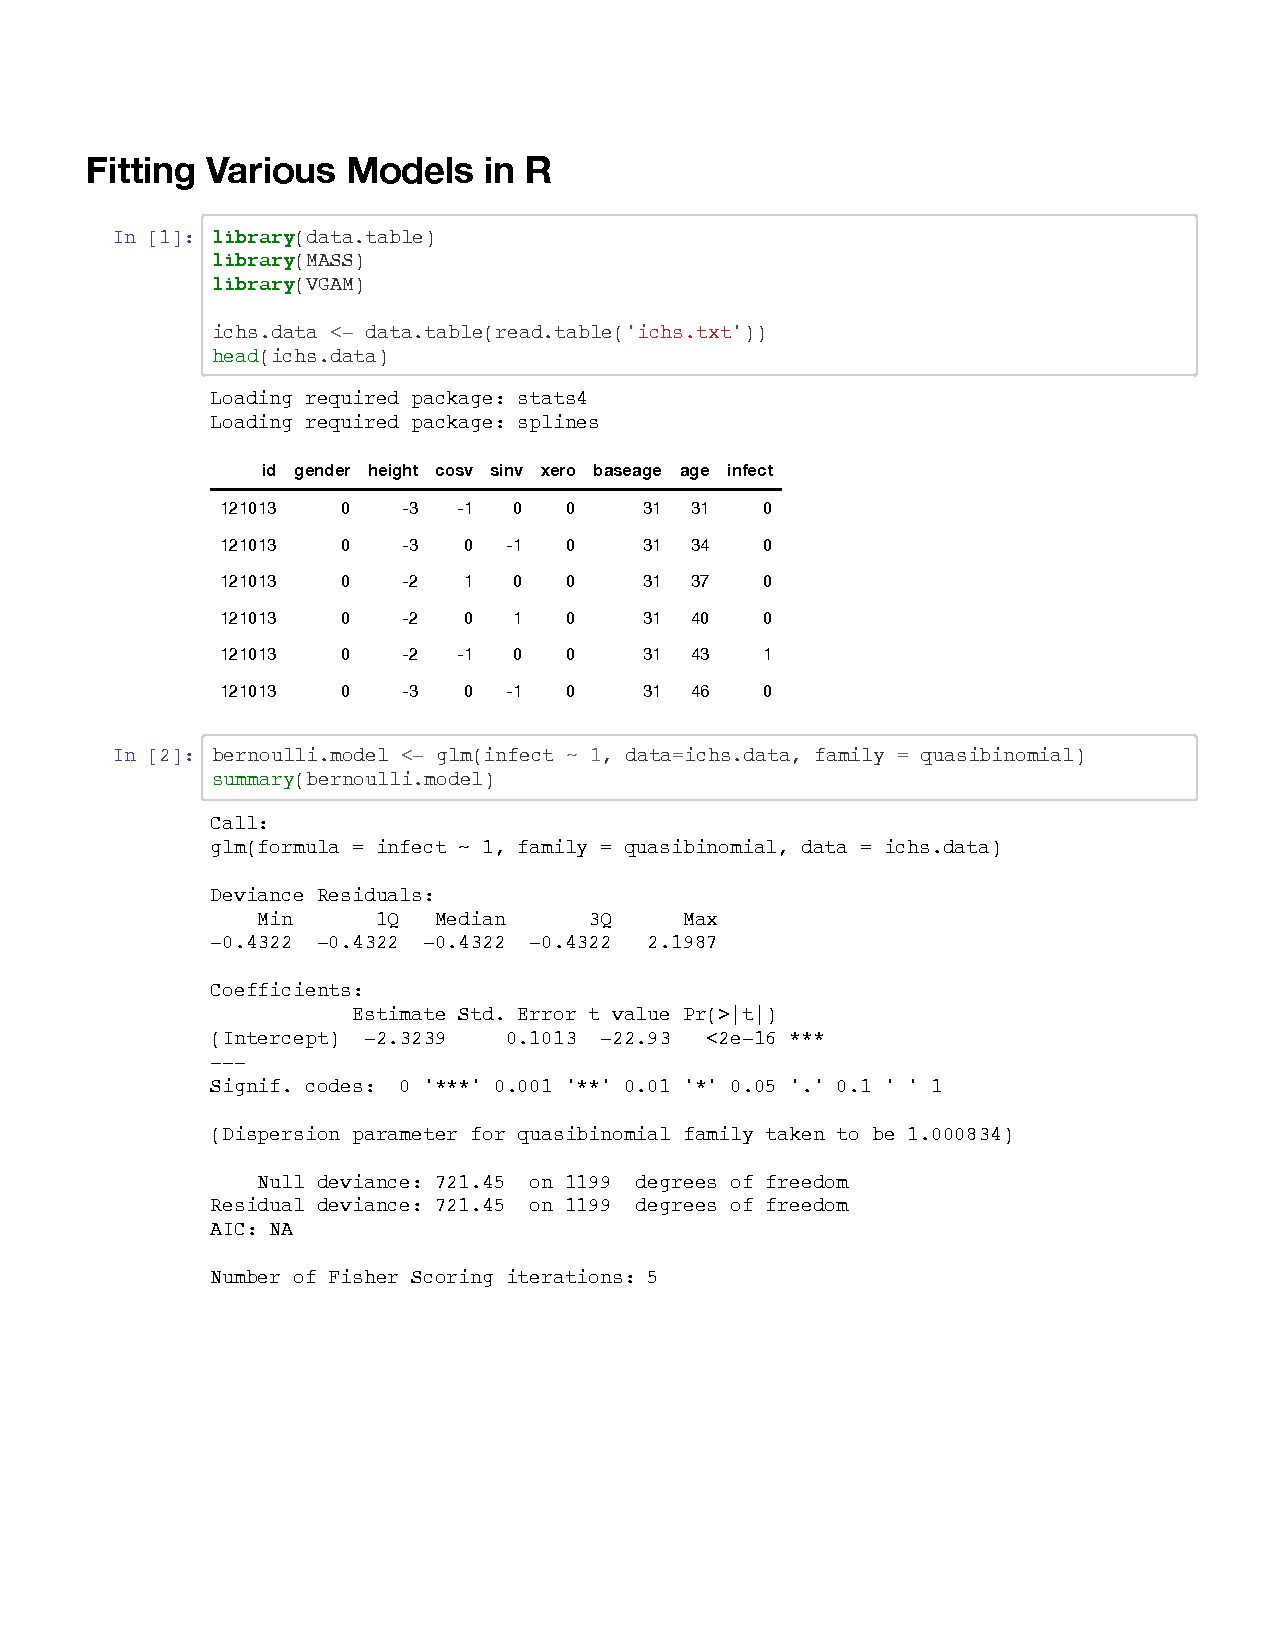
\includepdf[pages=-]{ichs_R.pdf}
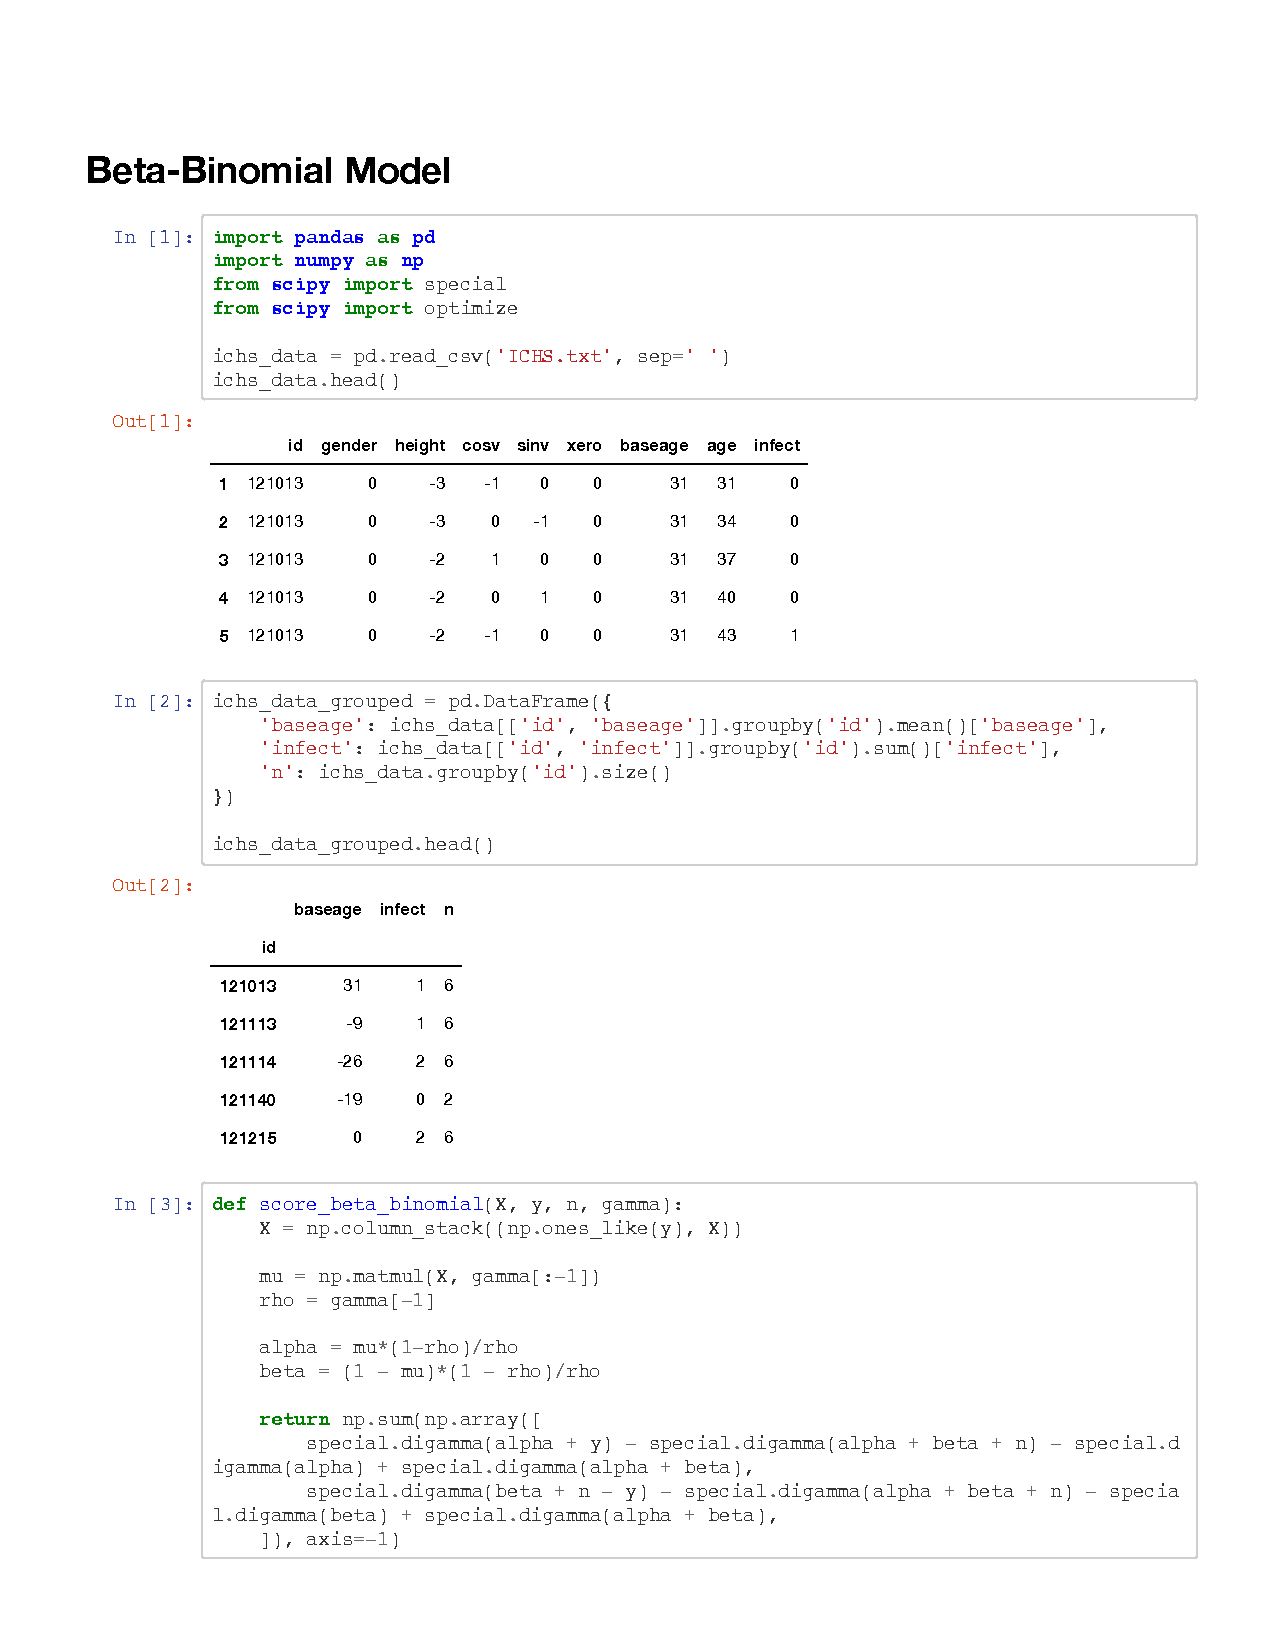
\includepdf[pages=-]{ichs_beta_binomial.pdf}

\end{document}